For the second iteration both the pathfinding and the raycasting had to be optimized since they both used to much of the CPU time.

\subsection*{Optimizing pathfinding}
A way to optimize pathfinding's runtime is to reduce the graph, this are done by remaking the grid graph to a waypoint graph.
The waypoint graph will be based on the outer corners of the obstacles on the map, where the AI had to make a turn, as seen in figure \ref{waypointsNode}.
Each point would then do a check on every other point to see if it was in direct sight, if that is the case it is added as a neighbour and the cost for that edge would be the euclidean distance to that point.
A resulting graph can be seen in Figure \ref{waypointgraph}.
In comparison to the old graph created had 3984 nodes and 30450 edges while this approach resulted in a much smaller graph with 47 nodes and 624 edges, thus improving both the creation of the graph and the traversal of it.

\begin{figure}[H]
\begin{center}
	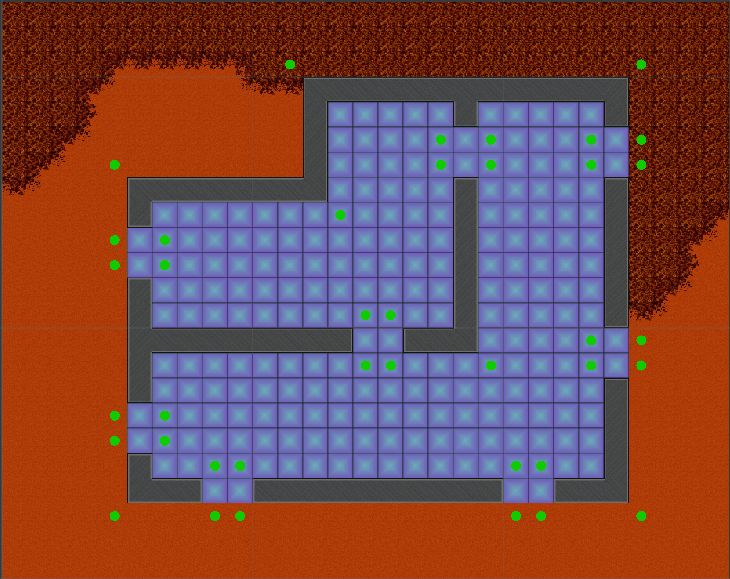
\includegraphics[width=0.5\textwidth]{figures/astar/waypoints}
	\caption{The placement of the waypoints}
	\label{waypointsNode}
	\end{center}
\end{figure}

\begin{figure}[H]
\begin{center}
	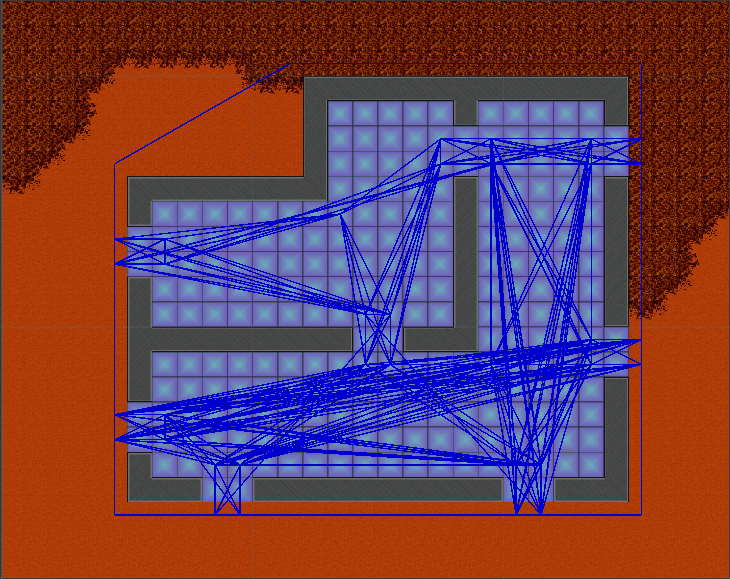
\includegraphics[width=0.5\textwidth]{figures/astar/waypointsGraph}
	\caption{Graph based on the waypoints}
	\label{waypointgraph}\end{center}
\end{figure}
This however raised a new problem, the problem consists of that since there were fewer waypoints available the enemies had to find the nearest accessible waypoint.
To solve this the distances was calculated to each waypoint from the given position and then a raycast was initiated towards the one with the smallest distance.
This raycast would have a maximum travel distance which would be the distance between the given position and the waypoint, if the raycast then returns an object it would mean there was something in the way. However, if nothing was returned would mean that there is a free path to the waypoint.
If the raycast returns an object the algorithm would move onto the second closest and so forth, as illustrated in Figure \ref{nearestWaypoint}.
\begin{figure}[H]
\begin{center}

	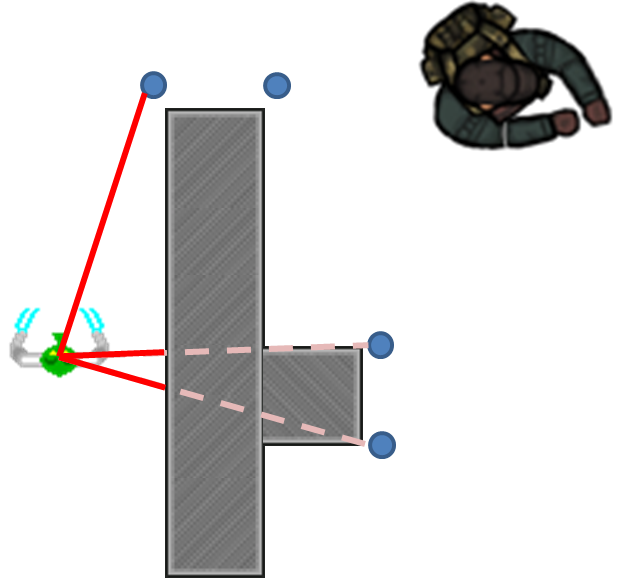
\includegraphics[width=0.4\textwidth]{figures/astar/findNearestWaypoint}
	\caption{Raycasts finding the nearest accessible waypoint}
	\label{nearestWaypoint}
	
\end{center}
\end{figure}

\subsection*{Minimizing of raycasting}
The minimizing of the raycasts is simply solved by adding a larger interval between each raycast.

\subsection*{Result}
This solution had a much better performance. However, we found that the raycasting still was too CPU intensive and desirable to remove it completely on runtime.